\section{Critical branching in detail}
\label{m:app:critical}

This appendix develops the critical theory of the binary Galton--Watson process
that \cref{m:sec:gw} summarises: the certainty of extinction at and below
criticality, the power-law survival and infinite expected lifetime at
criticality, and the total-progeny exponent. The asymptotics established here
are used again in the near-critical analysis of \ChA.

\subsection*{Certainty of extinction}
\label{m:sec:certainty}

Since $S_n$ is non-increasing and bounded below by $0$, it converges, and its
limit must be a fixed point of \cref{m:eq:SnIter}. Setting
$S_{n+1}=S_n=S_\infty$,
\begin{equation*}
S_\infty = 2pS_\infty - pS_\infty^2
\qquad\Longleftrightarrow\qquad
p\,S_\infty\lrb{S_\infty + \tfrac1p - 2} = 0 ,
\end{equation*}
with roots
\begin{equation*}
S_\infty = 0
\qquad\text{and}\qquad
S_\infty = 2-\frac1p = \frac{2p-1}{p} .
\end{equation*}
For $p<\tfrac12$ the second root is negative and carries no probabilistic meaning,
so the only admissible limit is $S_\infty=0$ and extinction is certain. At
$p=\tfrac12$ the two roots collide at the origin and extinction remains certain.
For $p>\tfrac12$ a positive root appears, and it is that root which is attained:
the process survives forever with positive probability
$S_\infty = (2p-1)/p$. \Cref{m:fig:phase_transition} shows the transition, together
with the change in stability of the origin that produces it.

\begin{figure}[htbp]
    \centering
    \begin{subfigure}[b]{0.31\textwidth}
        \centering
        \begin{tikzpicture}
            \begin{axis}[ch2plotstyle]
                \addplot[blue, thick] {2*0.3*x - 0.3*x^2};
                \addplot[black!45, dashed] {x};
                \addplot[only marks, mark=*, red, mark size=1.6pt] coordinates {(0,0)};
            \end{axis}
        \end{tikzpicture}
        \caption{Subcritical ($p = 0.3$)}
    \end{subfigure}
    \hfill
    \begin{subfigure}[b]{0.31\textwidth}
        \centering
        \begin{tikzpicture}
            \begin{axis}[ch2plotstyle]
                \addplot[blue, thick] {2*0.5*x - 0.5*x^2};
                \addplot[black!45, dashed] {x};
                \addplot[only marks, mark=*, red, mark size=1.6pt] coordinates {(0,0)};
            \end{axis}
        \end{tikzpicture}
        \caption{Critical ($p = 0.5$)}
    \end{subfigure}
    \hfill
    \begin{subfigure}[b]{0.31\textwidth}
        \centering
        \begin{tikzpicture}
            \begin{axis}[ch2plotstyle]
                \addplot[blue, thick] {2*0.74*x - 0.74*x^2};
                \addplot[black!45, dashed] {x};
                \addplot[only marks, mark=*, red, mark size=1.6pt] coordinates {(0,0) (0.64865,0.64865)};
            \end{axis}
        \end{tikzpicture}
        \caption{Supercritical ($p = 0.74$)}
    \end{subfigure}

    \vspace{10pt}
    \begin{subfigure}[b]{0.55\textwidth}
    \centering
    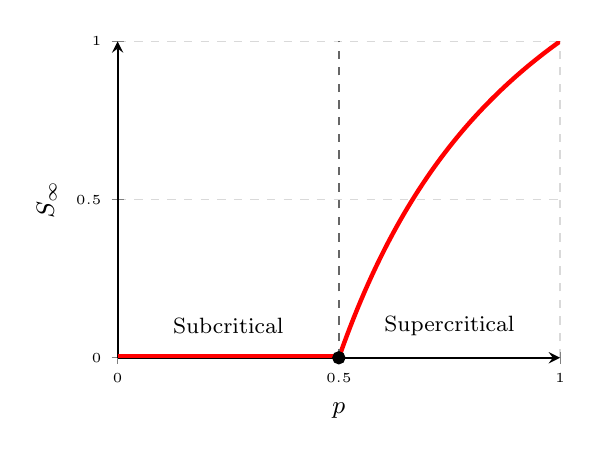
\begin{tikzpicture}
        \begin{axis}[
            width=7.2cm, height=5.6cm,
            axis lines=left,
            xlabel={$p$}, ylabel={$S_\infty$},
            xmin=0, xmax=1, ymin=0, ymax=1,
            xtick={0,0.5,1}, ytick={0,0.5,1},
            grid=major, grid style={dashed, gray!30}, thick,
            label style={font=\small}, tick label style={font=\tiny}
        ]
            \addplot[red, ultra thick, domain=0:0.5] {0.004};
            \addplot[red, ultra thick, domain=0.5:1, samples=120] {(2*x-1)/x};
            \draw[dashed, black!60] (axis cs:0.5,0) -- (axis cs:0.5,1);
            \node[font=\footnotesize] at (axis cs:0.25, 0.10) {Subcritical};
            \node[font=\footnotesize] at (axis cs:0.75, 0.10) {Supercritical};
            \addplot[only marks, mark=*, mark size=2pt, black] coordinates {(0.5,0)};
        \end{axis}
    \end{tikzpicture}
    \caption{The transition in $S_\infty$}
    \end{subfigure}

    \caption{Fixed points of the survival recursion \cref{m:eq:SnIter}. Panels
    (a)--(c) show the map $S\mapsto 2pS-pS^2$ (blue) against the diagonal (dashed),
    with the fixed points marked in red. Below and at criticality the origin is the
    only fixed point in $[0,1]$ and it is attracting, so extinction is certain; at
    $p=\tfrac12$ the map is tangent to the diagonal there. For $p>\tfrac12$ the
    origin turns repelling and a stable positive fixed point $S_\infty=(2p-1)/p$
    separates from it, traced in panel~(d).}
    \label{m:fig:phase_transition}
\end{figure}

\subsection*{The critical case: a power law and an infinite expected lifetime}
\label{m:sec:criticalcase}

At $p=\tfrac12$ the expectation is constant, $\ex{Z_n}=1$ for every $n$, and yet
extinction is certain. The two facts are reconciled by the tail: rare realisations
survive for enormously long times and grow enormously large, and they do so at
exactly the rate needed to hold the mean at one.

Let
\begin{equation*}
T = \inf\{n : Z_n = 0\}
\end{equation*}
be the extinction time, so that the process passes through generations
$0,1,\dots,T-1$ and is dead at $T$. Writing $T$ as a sum of indicators and taking
expectations term by term --- legitimate because every term is non-negative ---
\begin{equation}
\label{m:eq:ETsumSn}
\ex{T} = \sum_{n=0}^{\infty}\pr{T>n} = \sum_{n=0}^{\infty}\pr{Z_n>0}
= \sum_{n=0}^{\infty}S_n .
\end{equation}
The question is therefore how fast $S_n$ decays at criticality.

Setting $p=\tfrac12$ in \cref{m:eq:SnIter} gives $S_{n+1}-S_n = -\tfrac12 S_n^2$.
Once $n$ is large the unit generational increment is small compared with the scale
on which $S_n$ varies, and the difference on the left is well approximated by a
derivative. This step is heuristic --- it replaces a difference equation by a
differential one, and nothing here justifies the replacement beyond the smallness
of the increment relative to the solution --- but its conclusion is standard and is
confirmed by simulation below. With that caveat,
\begin{equation*}
\dda{S}{n} = -\tfrac12 S^2,
\qquad\text{with general solution}\qquad
S(n) = \frac{2}{n+\text{const}},
\end{equation*}
so that
\begin{equation}
\label{m:eq:twoovern}
S_n \sim \frac{2}{n}\qquad(n\to\infty),
\end{equation}
as \cref{m:fig:power_law}(a) confirms. The same asymptotic can in fact be obtained
directly from the exact recursion, without a continuum approximation: at
$p=\tfrac12$ the recursion reads $S_{n+1}=S_n(1-S_n/2)$, and since $S_n\downarrow0$
the reciprocal sequence has increments
\begin{equation}
\label{m:eq:reciprocalincrement}
\frac{1}{S_{n+1}}-\frac{1}{S_n}
= \frac{1}{2(1-S_n/2)} \;\longrightarrow\; \frac12 .
\end{equation}
Summing the convergent increments --- equivalently, applying the Stolz--Ces\`aro
theorem --- gives $(1/S_n)/n\to\tfrac12$, which is precisely
\cref{m:eq:twoovern}. This rigorous route, and the increment
\cref{m:eq:reciprocalincrement}, are used again in the near-critical analysis of
\ChA.

Substituting into \cref{m:eq:ETsumSn}, the tail of the sum behaves like twice the
harmonic series,
\begin{equation*}
\ex{T} = \sum_{n=0}^{\infty}S_n \sim \sum_{n=1}^{\infty}\frac{2}{n},
\end{equation*}
which diverges (\cref{m:fig:harmonic}). Since every $S_n$ is positive,
$\ex{T}=\infty$: the expected lifetime of the critical Galton--Watson process is
infinite even though extinction occurs with probability one. The point
probabilities of the lifetime follow from the exact decrement of the recursion:
\begin{equation}
\label{m:eq:Ttail}
\pr{T=n+1} = S_n - S_{n+1} = \tfrac12S_n^2 \sim \frac{2}{n^2},
\end{equation}
the heavy tail visible in \cref{m:fig:power_law}(b).

\begin{figure}[H]
    \centering
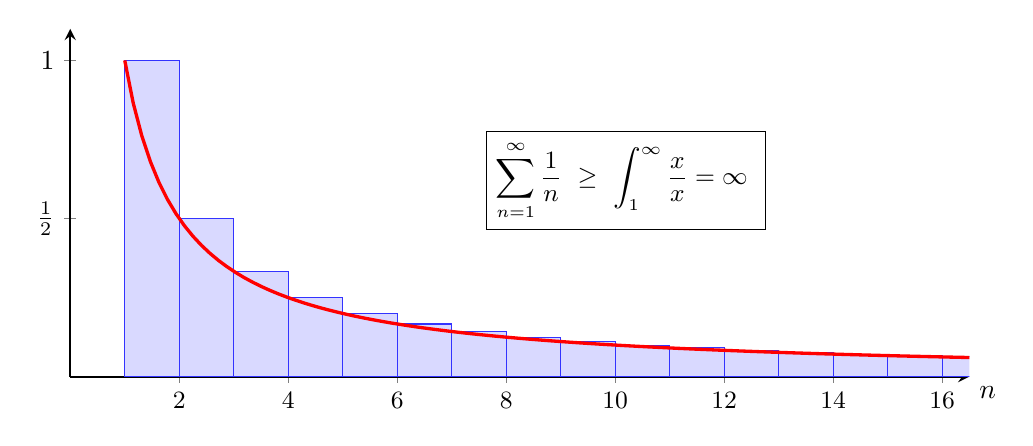
\begin{tikzpicture}
    \begin{axis}[
        axis lines = middle,
        xmin = 0, xmax = 16.5, ymin = 0, ymax = 1.1,
        xlabel = {$n$},
        xtick = {2,4,6,8,10,12,14,16},
        ytick = {0.5, 1}, yticklabels = {$\frac{1}{2}$, $1$},
        axis line style = {thick},
        width = 13cm, height = 6cm,
        every axis x label/.style={at={(current axis.right of origin)}, anchor=north west},
        xticklabel style={font=\small},
    ]
        \addplot[fill=blue!15, draw=blue!80, ybar interval, samples at={1,2,...,17}] {1/x} \closedcycle;
        \addplot[red, domain=1:16.5, samples=100, very thick] {1/x};
        \node[draw, fill=white, align=left, font=\small] at (axis cs: 10.2, 0.62) {
            $\displaystyle \sum_{n=1}^{\infty} \frac{1}{n} \ \ge\ \int_{1}^{\infty} \frac{\dd x}{x} = \infty$
        };
    \end{axis}
\end{tikzpicture}
\caption{Divergence of the harmonic series. Each blue rectangle has area $1/n$ and
contains the region under the red curve $1/x$ on $[n,n+1]$, so the sum of the areas
exceeds $\int_1^\infty x^{-1}\dd x=\infty$. Because $S_n\sim2/n$ at criticality,
the same divergence carries over to $\ex{T}=\sum_nS_n$.}
\label{m:fig:harmonic}
\end{figure}

A third critical exponent belongs to the total progeny
\begin{equation*}
\mathcal T = \sum_{n\ge0}Z_n ,
\end{equation*}
and it is worth recording because \cref{m:fig:power_law}(c) displays it. A finite
binary genealogy with $k$ division vertices has $k+1$ terminal vertices and hence
$2k+1$ individuals in all, and the number of such ordered full binary trees is the
Catalan number $C_k = (k+1)^{-1}\binom{2k}{k}$. Each division contributes a factor
$p$ and each death a factor $1-p$, so the exact law is
\begin{equation}
\label{m:eq:totalprogenyexact}
\pr{\mathcal T = 2k+1} = C_k\,p^k(1-p)^{k+1},
\end{equation}
zero at even values. At criticality Stirling's formula gives
\begin{equation}
\label{m:eq:totalprogenyasym}
\pr{\mathcal T = 2k+1} \sim \frac{1}{2\sqrt{\pi}}\,k^{-3/2},
\end{equation}
the classical $3/2$ law of critical branching, here along its admissible odd
support.

The heavy tail responsible for all of these exponents is visible directly in
simulation. A power-law distributed quantity carries a modest but non-negligible
chance of an extraordinarily large realisation, and a sample mean computed from
such a quantity does not settle: the larger the sample, the larger the mean,
because the occasional enormous value keeps pushing the normalised sum upward.
\Cref{m:fig:power_law} collects the three classical critical exponents --- for the
survival probability, for the extinction time and for the total progeny.

\begin{figure}[ht]
    \centering
    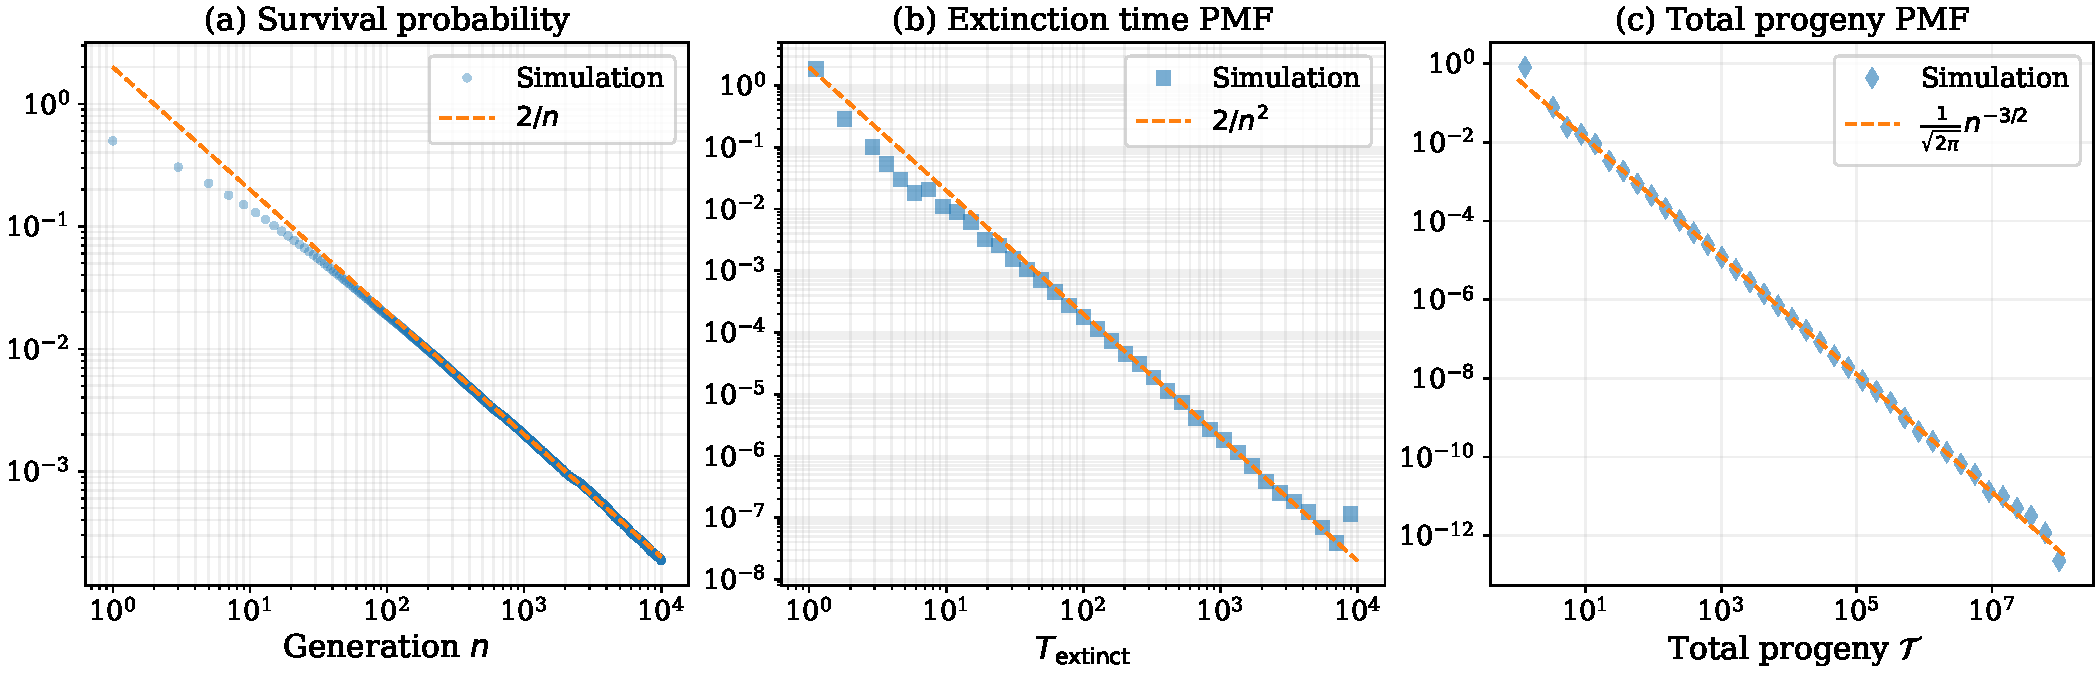
\includegraphics[width=0.98\textwidth]{figures/power_law_fixed.pdf}
    \caption{Power-law behaviour in the critical Galton--Watson process
    ($p=0.5$), from $10^6$ realisations.
    (a) Survival probability $S_n=\pr{Z_n>0}$, showing the late-generation scaling
    $S_n\sim2/n$ of \cref{m:eq:twoovern}.
    (b) Probability mass function of the extinction time $T=\inf\{n:Z_n=0\}$, with
    heavy tail $\pr{T=n}\sim2/n^2$ as in \cref{m:eq:Ttail}.
    (c) Probability mass function of the total progeny
    $\mathcal T = \sum_{k\ge0}Z_k$, displaying the classical critical branching
    asymptotic $\pr{\mathcal T=n}\sim n^{-3/2}$ of \cref{m:eq:totalprogenyasym}.}
    \label{m:fig:power_law}
\end{figure}

\FloatBarrier
